\subsection{Task 1.1.2: Radial Basis Functions}


\subsubsection{Aufgabenstellung:}
Nun ist die Basisfunktion eine Gau\ss{} 'sche Glockenkurve die mit $\phi_k(x) = exp(-(x-\mu_k)^2 /\sigma^2 )$ gegeben ist.
Wobei $d=2:18$, $\sigma$ $= 2/d$ und $\mu =d$ schritten zwischen -1 und 1 entspricht.
Es sind wieder  die Trainingspunkte, die Target-Funktion(y\_target) und die ``Lernfunktionen'' zu Auszugeben.
Die Basisfunktion mit $d=6,12$ und $18$ als Funktion von x zu Ploten.
Ausgeben des ``Mean Squared Error'' (MSE) für die Trainings- und Test- werte.



\subsubsection{Plots \& Diskussion:}


\begin{figure}[hp!]
\begin{center}
 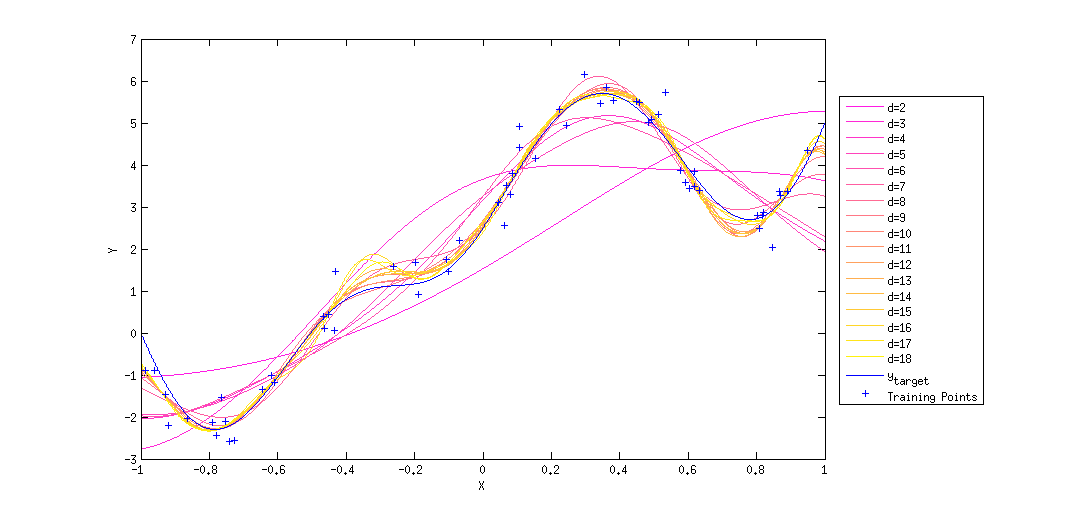
\includegraphics[width=1\textwidth]{./figures/RBF_learn}
 \caption[Trainingspunkte, Target-Funktion und Lernfunktionen]{Trainingspunkte, Target-Funktion und Lernfunktionen}
\label{fig:RBF_learn}
\end{center}
\end{figure}
Wie man in Abb. \ref{fig:RBF_learn} sehen kann ist das ``Ausbrechen'' bei der Radial-Funktion, am Ende, bei weitem nicht so ausgeprägt!

\begin{figure}[hp!]
\begin{center}
 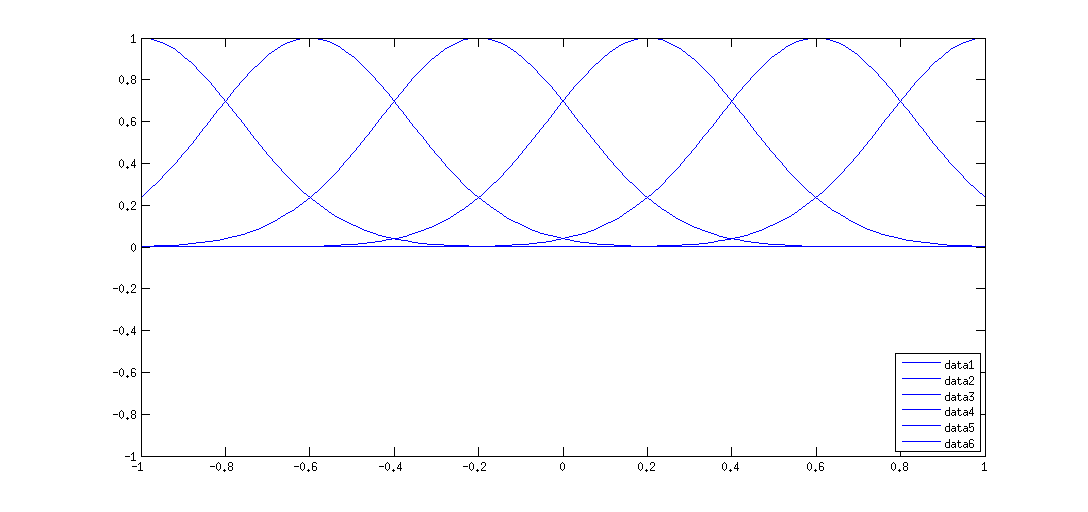
\includegraphics[width=10cm]{./figures/RBF_6}
 \caption[Basisfunktionen als Funktion von X (d=6)]{Basisfunktionen als Funktion von X mit einem $d=6$}
\label{fig:RBF_6}
\end{center}
\end{figure}

\begin{figure}[hp!]
\begin{center}
 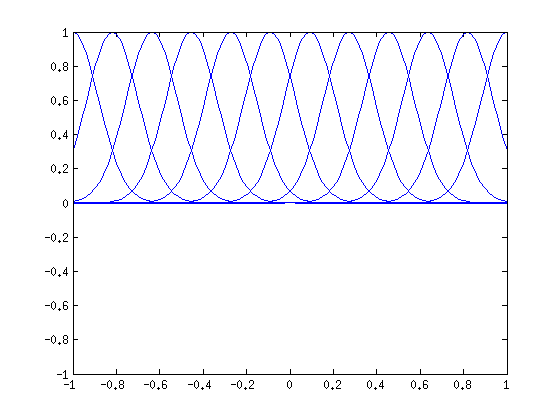
\includegraphics[width=10cm]{./figures/RBF_12}
 \caption[Basisfunktionen als Funktion von X, d=12]{Basisfunktionen als Funktion von X mit einem $d=12$}
\label{fig:RBF_12}
\end{center}
\end{figure}


\begin{figure}[hp!]
\begin{center}
 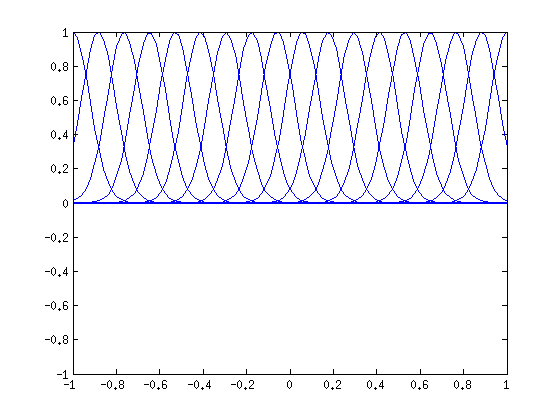
\includegraphics[width=10cm]{./figures/RBF_18}
 \caption[Basisfunktionen als Funktion von X, d=18]{Basisfunktionen als Funktion von X mit einem $d=18$}
\label{fig:RBF_18}
\end{center}
\end{figure}
Man kann erkennen das auch hier bei höherer Ordnung die Steilheit zunimmt. Gau\ss{}'sche-funktionen neigen allerdings nicht zum ``ausbrechen''
da sie wenn sie Richtung unendlich gehen keinen ``Schaden'' anrichten, da sie wieder zu ihrem Nullpunkt zurückkehren.
Was sich auch in Abb. \ref{fig:RBF_MSE} zeigt, da hier der MSE der Test-Werte, bei hohem Grad nicht stark ansteigt wie in Bsp.1.1.1.
 

\begin{figure}[hp!]
\begin{center}
 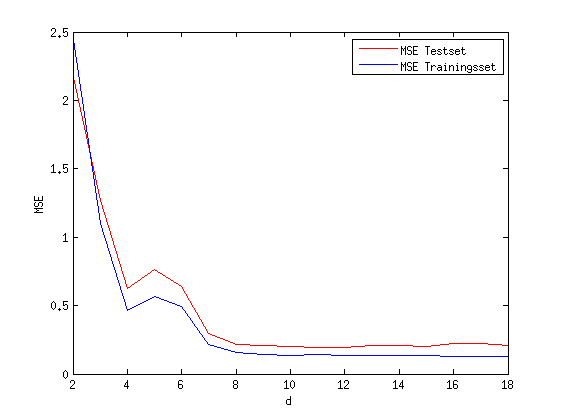
\includegraphics[width=10cm]{./figures/RBF_MSE}
 \caption[MSE]{MSE des Trainingsset und des Testsets.}
\label{fig:RBF_MSE}
\end{center}
\end{figure}
\clearpage